% Adjust these for the path of the theme and its graphics, relative to this file
%\usepackage{beamerthemeFalmouthGamesAcademy}
\usepackage{../../beamerthemeFalmouthGamesAcademy}
\usepackage{multimedia}
\graphicspath{ {../../} }

% Default language for code listings
\lstset{language=C++,
        morekeywords={each,in,nullptr,int32, TCHAR, uint8, int8, uint16, int16,
        uint32, int32, uint64, int64, PTRINT, UObject. AActor, SWidget, FName,
        FString, UClass, USoundCue, UTexture}
}

% For strikethrough effect
\usepackage[normalem]{ulem}
\usepackage{wasysym}
\usepackage{listings}
\usepackage{pdfpages}

% http://www.texample.net/tikz/examples/state-machine/
\usetikzlibrary{arrows,automata}

\newcommand{\modulecode}{COMP260}\newcommand{\moduletitle}{Distributed Systems}\newcommand{\sessionnumber}{5}

\begin{document}
\title{\sessionnumber: Memory}
\subtitle{\modulecode: \moduletitle}

\frame{\titlepage}

\begin{frame}
	\frametitle{Learning outcomes}
	\begin{itemize}
		\item \textbf{Understand} Memory in modern object orientated languages
		\item \textbf{Compare} memory models in managed and unmanaged languages
		\item \textbf{Understand} the role of the profiler in measuring performance in games
	\end{itemize}
\end{frame}

\part{Memory}
\frame{\partpage}

\begin{frame}{Memory Refresher}
	\begin{itemize}
		\pause \item Recall that:
		\begin{itemize}
			\pause \item Dynamic memory, allocated on the \textbf{Heap} and is \textbf{growable}
			\pause \item Static memory, allocated on the \textbf{Stack} and is \textbf{fixed size}
		\end{itemize}
	\end{itemize}
\end{frame}

\begin{frame}{Stack Memory}
	\begin{itemize}
		\pause \item When you allocate value types (int, float, short, char etc), these are allocated on the stack
		\pause \item Values allocated on the stack are local, when they drop out of scope they are deallocated  
		\pause \item Values passed into functions are copied onto the stack
		\pause \item The stack is of fixed size
		\begin{itemize}
			\item C++ Visual Studio - \textbf{1MB}
		\end{itemize}
	\end{itemize}
\end{frame}

\begin{frame}[fragile]{Stack Memory Example 1}
	\begin{lstlisting}
		void Update()
		{
			int x=10;
			int y=10;
	
			Vector2 pos=Vector2(x,y);
		} //<-- x, y and pos drop out of scope here
	\end{lstlisting} 
\end{frame}

\begin{frame}[fragile]{Stack Memory Example 2}
	\begin{lstlisting}[language=C++,basicstyle=\tiny,]
		class MonsterStats
		{
		private:
			int health;
			int strength;
		public:
			MonsterStats()
			{
				health=100;
				strength=10;
			};
	
			void ChangeHealth(int h)
			{
				health+=h;
			};//<- h drops out of scope here
	
			void ChangeStrength(int s)
			{
				strength+=s;
			};//<- s drops out of scope here
		};
	
		void main()
		{		
			//Create an instance of the class on the stack
			MonsterStats stats=MonsterStats();
			stats.ChangeHealth(10);
			stats.ChangeStrength(-2);
		}//<-- stats drops out of scope here
	\end{lstlisting}
\end{frame}

\begin{frame}{Heap Memory}
	\begin{itemize}
	\pause \item Otherwise known as dynamic memory
	\pause \item Types allocated with the \textbf{new} keyword are allocated on the heap
	\pause \item The new operator returns a reference to the type and can be allocated to a pointer (C++)
	\pause \item This heap is managed by the programmer in C++ (see \textbf{delete} keyword) or the garbage collector in C\#
	\pause \item In C++ is very important that you delete anything allocated on the heap
	\pause \item \textbf{for every new, you need a matching delete}
	\pause \item In the Unreal Engine objects can be Garbage Collected
	\end{itemize}
\end{frame}


\begin{frame}[fragile]{Heap Memory Example 1 - C++}
\begin{lstlisting}[language=C++,basicstyle=\tiny,]
	class MonsterStats
	{
	private:
		int health;
		int strength;
	public:
		MonsterStats()
		{
			health=100;
			strength=10;
		}
		
	.....
	}
	
	void main()
	{		
		//Create an instance of the class on the Heap
		MonsterStats * stats=new MonsterStats();
		stats->ChangeHealth(10);
		stats->ChangeStrength(-2);
	
		if (stats)
		{
		delete stats;
		stats=nullptr;
		}
	}
\end{lstlisting}
\end{frame}

\begin{frame}{Passing Variable}
	\begin{itemize}
		\pause \item In C++, we can pass by value or reference. In addition to this, we can also pass in a pointer
		\pause \item We can mark parameter with \textbf{\&} to pass by Reference 
		\pause \item Custom data types and strings should be passed by Pointer or Reference
	\end{itemize}
\end{frame}

\begin{frame}[fragile]{Passing Example 1 - C++}
	\begin{lstlisting}
		int x=10;
	
		void Adder(int &value,int v)
		{
			value+=v;	
		}
	
		Adder(x,10);
		//x would now be 20 after this		
	
	\end{lstlisting}
\end{frame}

\begin{frame}[fragile]{Passing Example 2 - C++}
	\begin{lstlisting}
	
		void SetupMonster(MonsterStats &stats, int health, int strength)
		{
			stats.health=health;
			stats.strength=strength;
		}
		
		//Calling code
		MonsterStats * goblinStats=new MonsterStats();
		SetupMonster(goblinStats,10,2);
	\end{lstlisting}
\end{frame}


\part{String types}
\frame{\partpage}

\begin{frame}{Strings}
	\begin{itemize}
		\pause\item A \textbf{string} represents a sequence of textual characters
		\pause\item E.g.\ \lstinline{"Hello world!"}
		\pause\item C\# type: \csinline{string}
		\pause\item Python type: \pyinline{str}
	\end{itemize}
\end{frame}

\begin{frame}{String representation}
	\begin{itemize}
		\pause\item Stored as sequences of \textbf{characters} encoded as \textbf{integers}
		\pause\item Often \textbf{null-terminated}
			\begin{itemize}
				\pause\item Character number 0 signifies the end of the string
			\end{itemize}
	\end{itemize}
\end{frame}

\begin{frame}{What is a character?}
	\begin{itemize}
		\pause\item Broadly speaking, a single \textbf{printable symbol} or \textbf{glyph}
		\pause\item (Actually a lot more complicated than this, but this will do for today)
		\pause\item There are also some special \textbf{non-printable characters} e.g.\ line break
	\end{itemize}
\end{frame}

\begin{frame}{ASCII}
	\begin{itemize}
		\pause\item American Standard Code for Information Interchange
		\pause\item Defines a standard set of 128 characters (7 bits per character)
		\pause\item Originally developed in the 1960s for teletype machines, but survives in computing to this day
		\pause\item 95 printable characters: upper and lower case English alphabet, digits, punctuation
		\pause\item 33 non-printable characters
	\end{itemize}
\end{frame}

{
\setbeamercolor{background canvas}{bg=white}
\begin{frame}[plain]
	\begin{tikzpicture}[remember picture, overlay]
		\node[at=(current page.center)] {
			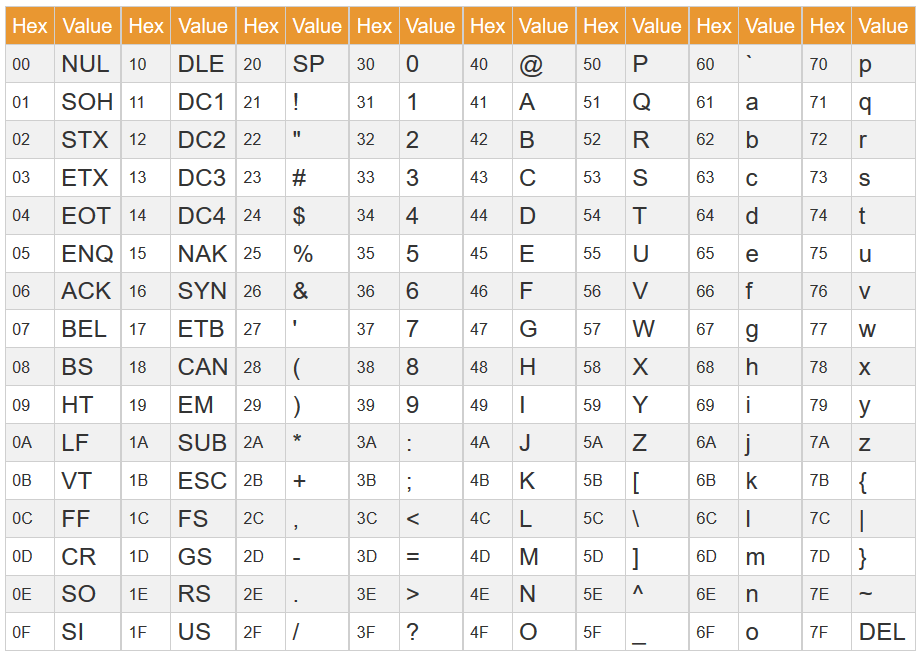
\includegraphics[width=\paperwidth]{ascii_chart_2}
		};
	\end{tikzpicture}
\end{frame}
}

\begin{frame}{ASCII}
	\begin{itemize}
		\pause\item ASCII works OK for English
		\pause\item Standards exist to add another 128 characters (taking us to 8 bits per character)
		\pause\item E.g.\ accented characters for European languages, other Western alphabets e.g. Greek, Cyrillic,
		    mathematical symbols
		\pause\item However 256 characters isn't enough...
	\end{itemize}
\end{frame}

\begin{frame}{Unicode}
	\begin{itemize}
		\pause\item Standard character set developed from 1987 to present day
		\pause\item Currently defines 144697 characters (Unicode 14.0)
		\pause\item First 128 characters are the same as ASCII
		\pause\item Covers most of the world's writing systems
		\pause\item Also covers mathematical symbols and emoji
	\end{itemize}
\end{frame}

\begin{frame}{Encoding Unicode}
    \begin{itemize}
		\pause\item \textbf{UTF-32} encodes characters as 32-bit integers
		\pause\item \textbf{UTF-8} encodes characters as 8, 16, 24 or 32-bit integers
			\begin{itemize}
			    \pause\item 8-bit characters correspond to the first 128 ASCII characters
			        $\implies$ backwards compatible
				\pause\item More common Unicode characters are smaller
				    $\implies$ more efficient than UTF-32
			\end{itemize}
	\end{itemize}
\end{frame}

% \begin{frame}{String representation}
% 	\begin{itemize}
% 		\pause\item \lstinline{"Hello world!"} in ASCII or UTF-8 encoding:
% 	\end{itemize}
	
% 	{\footnotesize\pause\begin{tabular}{*{13}{|c}|}
% 		\hline
% 		72 & 101 & 108 & 108 & 111 & 32 & 119 & 111 & 114 & 108 & 100 & 33 & 0 \\\hline
% 	\end{tabular}}
% \end{frame}

\begin{frame}{UTF-8 representation}
	\begin{itemize}
		\pause\item For characters in ASCII, UTF-8 is the same:
			\begin{itemize}
				\pause\item a $\to [97]$
			\end{itemize}
		\pause\item Other characters are encoded as multi-byte sequences:
			\begin{itemize}
				\pause\item \"u $\to [195, 188]$
				\pause\item 
\includegraphics[height=1.5ex]{chinese}\ $\to [229, 150, 130]$
				\pause\item 
\includegraphics[height=1.5ex]{emoji}\ $\to [240, 159, 152, 130]$
			\end{itemize}
		\pause\item \texttt{"Haha 
\includegraphics[height=1.5ex]{emoji}"} encoded in UTF-8:
	\end{itemize}
	{\footnotesize\pause\begin{tabular}{*{13}{|c}|}
		\hline
		H & a & h & a & space & \multicolumn{4}{c|}{
\includegraphics[height=1.5ex]{emoji}} & null \\\hline
		72 & 97 & 104 & 97 & 32 & 240 & 159 & 152 & 130 & 0 \\\hline
	\end{tabular}}
\end{frame}

% \begin{frame}{Strings in Python}
%     \begin{itemize}
%         \pause\item Python 2 had separate types for ASCII and Unicode strings: \lstinline{str} and \lstinline{unicode}
%         \pause\item Python 3 has just the \lstinline{str} type, which uses Unicode
%         \pause\item String literals are wrapped in \lstinline{'single quotes'} or \lstinline{"double quotes"}
%             (there is no difference)
%     \end{itemize}
% \end{frame}

\begin{frame}[fragile]{Escape sequences}
    \begin{itemize}
        \pause\item Backslash \textbackslash\ has a special meaning in string literals
            --- it denotes the start of an \textbf{escape sequence}
        \pause\item Typically used to write \textbf{non-printable characters}
        \pause\item Most useful: \lstinline{"\n"} is a new line
        \pause\item How to type a backslash character? Use \lstinline{"\\"}
    \end{itemize}
\end{frame}

% \begin{frame}{String literal tricks in Python}
%     \begin{itemize}
%         \pause\item Use triple quotes \lstinline{'''} or \lstinline{"""} for a multi-line string
%         \pause\item Use \lstinline{r" "} or \lstinline{r' '} to turn off escape characters
%             (useful for strings with lots of backslashes, e.g.\ Windows file paths, regular expressions)
%     \end{itemize}
% \end{frame}

\begin{frame}[fragile]{Text files}
    \begin{itemize}
        \pause\item Stored on disk as essentially one long string
        \pause\item Line endings are denoted by non-printable characters
            \begin{itemize}
                \pause\item Unix format: line feed character (ASCII/UTF-8 character 10, \lstinline{"\n"})
                \pause\item Windows format: carriage return character (ASCII/UTF-8 character 13) followed by line feed, \lstinline{"\r\n"}
                \pause\item Most text editors can handle and convert both formats
                \pause\item Most languages allow files to be opened in ``text mode'' which automatically converts
            \end{itemize}
    \end{itemize}
\end{frame}


\part{Memory Management}
\frame{\partpage}

\begin{frame}
\frametitle{Garbage Collection in C\#}
\begin{itemize}
	\item In C\# there is an inbuilt Garbage Collector which will  walk through the Object Graph
	\item It will check to see if the object is still allocated, if not, the Garbage Collector will cleanup the object
	\item This process is automatic and is tuned for maximum performance
	\item However you should think of caching GetComponent calls using the \textbf{Start} or \textbf{Awake}
\end{itemize}
\end{frame}

\begin{frame}
\frametitle{Memory Management in C++}
\begin{itemize}
\item In C++ there is no Garbage Collection, you have to manually delete objects when no longer needed
\item Worth repeating  \textbf{for every new, you need a matching delete}
\end{itemize}
\end{frame}

\part{Exercises}
\frame{\partpage}

\begin{frame}{Exercise 1 - Texturing}
	\begin{itemize}
		\item Load in a image using SDL Image
		\item Copy this image into a OpenGL Texture
		\item Add Texture Coordinates to your Cube or Square
		\item Map this texture onto the Cube or Square
		\item Finally change the texture to a transparent texture
	\end{itemize}
\end{frame}

\begin{frame}{Exercise 2 - Model Loading}
	\begin{itemize}
		\item Create the following NFF models and load each one to the screen
		\begin{itemize}
			\item Tetrahedron 
			\item Cube
			\item Sphere
			\item Cylinder
		\end{itemize}
		\item \url{http://assimp.sourceforge.net/howtoBasicShapes.html}
		\item \url{https://github.com/assimp/assimp/tree/master/test/models/NFF/NFF}
	\end{itemize}
\end{frame}

\begin{frame}{Exercise 3 - More Complex Scene}
	\begin{itemize}
		\item Create a GameObject class which contains the following as member variables
		\begin{itemize}
			\item Vertex Buffer
			\item Element Buffer
			\item Vertex Array Object
			\item Position, Scale, Rotation Vectors
			\item Position, Scale, Rotation, Model Matrices
			\item Open GL Texture
			\item Number of vertices and Indices
		\end{itemize}
		\item Add in functions to initialise and get each of these values
		\item Add in functions to update (calculate the model matrix) and render
		\item Create an instance of this Game Object and display it on the screen
	\end{itemize}
\end{frame}

\end{document}
